\section{Saturation and weak bisimulation equivalence}
% no \IEEEPARstart
Def: Let $P$ and $Q$ be CCS processes or, more generally, states in a labeled transition system. For each action $a$, we shall write
$P\stackrel{a}{\Rightarrow}Q$ iff:
\begin{itemize}
	\item Either $a\neq\tau$ and there are processes $P'$ and $Q'$ such that $P\left(\stackrel{\tau}{\rightarrow}\right)^{*}P'\ \stackrel{a}{\rightarrow}\ Q'\left(\stackrel{\tau}{\rightarrow}\right)^{*}Q$,
	\item Or $a=\tau$ and $P\left(\stackrel{\tau}{\rightarrow}\right)^{*}Q$,
\end{itemize}
where we write $\left(\stackrel{\tau}{\rightarrow}\right)^{*}$ for he reflexive and transitive closure of the relation $\stackrel{\tau}{\rightarrow}$.

Def: (weak bisimulation and observational equivalence) A binary relation $R$ over the set of states of an LTS is a weak bisimulation iff, whenever $s_{1}Rs_{2}$ and $a$ is an action (including $\tau$):
\begin{itemize}
	\item If $s_{1}\stackrel{a}{\rightarrow}s_{1}'$ then there is a transition $s_{2}\stackrel{a}{\Rightarrow}s_{2}'$ such that $s_{1}'Rs_{2}'$;
	\item If $s_{2}\stackrel{a}{\rightarrow}s_{2}'$ then there is a transition $s_{1}\stackrel{a}{\Rightarrow}s_{1}'$ such that $s_{1}'Rs_{2}'$;
\end{itemize}

Two states $s$ and $s'$ are observationally equivalent (or weakly bisimilar), written $s\approx s'$, iff there is a weak bisimulation equivalence that relates them.

Def: Let $T\subseteq S\times Act\times S$ be an LTS. We shall say that\\ 
$T^{*}=\left\{\left(p,a,q\right)| p\stackrel{a}{\Rightarrow}q\right\}=T\cup\left(\stackrel{a}{\rightarrow}\right)^{*}\cup\left\{\left(p,a,q\right)| a\neq\tau\wedge\left(\exists p',q'\in A\right) p\left(\stackrel{\tau}{\rightarrow}\right)^{*}p'\stackrel{a}{\rightarrow}q'\left(\stackrel{\tau}{\rightarrow}\right)^{*}q\right\}$ is a saturation of T.

Proposition: Two LTSs are weakly bisimilar iff their saturated LTSs are strongly bisimilar. 

Proof: Let $T$ and $U$ be two LTSs for which their saturated LTSs are strongly bisimilar by the relation $R$. Since the strong bisimulation is also a weak bisimulation it follows that $T$ and $U$ are weakly bisimular, since they are weakly bisimular to their respective saturated LTSs.
Let $T$ and $U$ be two LTSs that are weakly bisimilar. Let $u\approx t$, $u'\approx t'$. If $t\stackrel{a}{\rightarrow}t'\in T^{*}$, that means $t\stackrel{a}{\Rightarrow}t'$, or that there exist states $t_{i}$, $t'_{j}$ such that: $t\stackrel{\tau}{\rightarrow}t_{1}\stackrel{\tau}{\rightarrow}...\stackrel{\tau}{\rightarrow}t_{k}\stackrel{a}{\rightarrow}t'_{1}\stackrel{\tau}{\rightarrow}...\stackrel{\tau}{\rightarrow}t'_{m}\stackrel{\tau}{\rightarrow}t'$. Let $u_{i}\approx t_{i}$,...,$u'_{j}\approx t'_{j}$,.... It follows that $u\stackrel{\tau}{\Rightarrow}u_{1}\stackrel{\tau}{\Rightarrow}...\stackrel{\tau}{\Rightarrow}u_{k}\stackrel{a}{\Rightarrow}u'_{1}\stackrel{\tau}{\Rightarrow}...\stackrel{\tau}{\Rightarrow}u'$, or that there exist states $u''$, $u'''$ in U such that $u\left(\stackrel{\tau}{\rightarrow}\right)^{*}u_{k}\left(\stackrel{\tau}{\rightarrow}\right)^{*}u''\stackrel{a}{\rightarrow}u'''\left(\stackrel{\tau}{\rightarrow}\right)^{*}u'_{1}\left(\stackrel{\tau}{\rightarrow}\right)^{*}u'$ which means $u\stackrel{a}{\Rightarrow}u'$. Since $U^{*}$ is a saturation of $U$, it follows that $u\stackrel{a}{\rightarrow}u'\in U^{*}$.
Similarly, for every transition $u\stackrel{a}{\rightarrow}u'\in U^{*}$, there is a transition in $t\stackrel{a}{\rightarrow}t'\in T^{*}$, such that $u\approx t$, $u'\approx t'$.
Therefore, the weak bisimulation relation $\approx$ for $T$ and $U$ is a strong bisimulation relation for $T^{*}$ and $U^{*}$.

\subsection{The algorithm for saturation.}

The set of triples ${R}$ can be partitioned in ${2n}$ sets with: \\
\ \ \ \ ${T_{\tau p}=\left\{\left(p,\tau,q\right)| \left(p,\tau,q\right)\in T\right\}}$, and\\
\ \ \ \ ${T_{ap}=\left\{\left(p,\tau,q\right)|\ a\neq\tau\wedge\left(p,\tau,q\right)\in T\right\}}$ for every ${p\in S}$.

By the definition of ${T_{\tau p}}$ and ${T_{ap}}$ it can be seen that ${\bigcup_{p\in S}\left(T_{\tau p}\cup T_{ap}\right)=T}$, and also, their pairwise intersection is empty. 

The family of sets ${T^{*}_{\tau p}}$ can be iteratively constructed with:\\
${T^{0}_{\tau p}=T_{\tau p}\cup\left\{\left(p,\tau,p\right)\right\}}$,\\
${T^{i}_{\tau p}=T^{i-1}_{\tau p}\cup\left\{\left(p,\tau,r\right)|\left(\exists q\in S\right)\left(p,\tau,q\right)\in T^{i-1}_{\tau p}\wedge\left(q,\tau,r\right)\in T_{\tau q}\right\}}$ and \\
${T^{*}_{\tau p}=T^{n}_{\tau p}}$

(Note: ${\left|T^{*}_{\tau p}\right|\leq\left|S\right|=n}$; when for some ${k<n}$, ${T^{k}_{\tau p}=T^{k+1}_{\tau p}}$, then ${T^{*}_{\tau p}=T^{k}_{\tau p}=T^{n}_{\tau p}}$)

With this step a reflexive, transitive closure was constructed: ${T^{*}_{\tau}=\bigcup_{p\in A}T^{*}_{\tau p}=\left\{\left(p,\tau,q\right)|p\left(\stackrel{\tau}{\rightarrow}\right)^{*}q\right\}}$.

\begin{figure}[!ht]
\centering
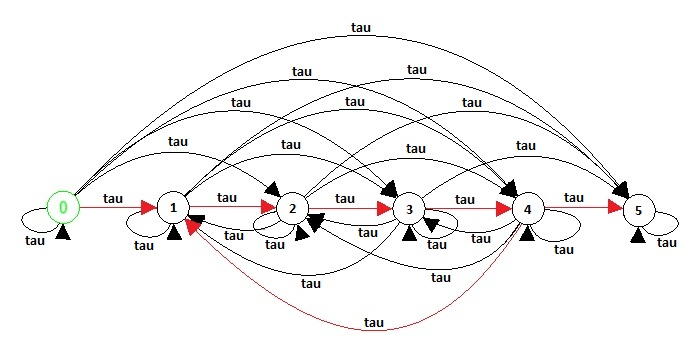
\includegraphics[width=4.5in]{saturation}
\caption{Reflexive, transitive closure of $\tau$. The original graph is depicted with red lines}
\label{fig:saturation}
\end{figure}

The next step is to construct $T'_{ap}=\bigcup_{p\in A}T'_{ap}=\left\{\left(p,a,q\right)|\left(\exists q'\in S\right)\left(p,a,q'\right)\in T\wedge q'\left(\stackrel{\tau}{\rightarrow}\right)^{*}q\right\}$:\\
$T^{0}_{ap}=T_{ap'}$,\\
$T^{i}_{ap}=T^{i-1}_{ap}\cup \left\{\left(p,a,r\right)|\left(\exists q\in S\right)\left(p,a,q\right)\in T^{i-1}_{ap}\wedge \left(q,\tau,r\right)\in T^{i-1}_{\tau q}\right\}$ and \\
$T'_{ap}=T^{n|Act|}_{ap}$

(Note: $|T'_{ap}|\leq |S||Act|=n|Act|$, when for some $k<n|Act|$, $T^{k}_{ap}=T^{k+1}_{ap}$, then $T'_{ap}=T^{k}_{ap}=T^{n|Act|}_{ap}$)

For the third step, $T'=\bigcup_{p\in S}\left(T^{*}_{\tau p}\cup T'_{ap}\right)$ needs to be partitioned again, defined by the destination in the triple:\\
$T_{\tau q}=\left\{\left(p,\tau,q\right)|\left(p,\tau,q\right)\in T'\right\}$ and $T_{bq}=\left\{\left(p,a,q\right)|a\neq\tau\wedge\left(p,a,q\right)\in T'\right\}$ for every $p\in S$,\\
and then construct:\\
$T^{0}_{bq}=T_{bq}$,\\
$T^{i}_{bq}=T^{i-1}_{bq}\cup\left\{\left(p',a,q\right)|\left(\exists p\in S\right)\left(p,a,q\right)\in T^{i-1}_{bq}\wedge\left(p',\tau,p\right)\in T^{*}_{\tau p}\right\}$ and\\
$T^{*}_{bq}=T^{n|Act|}_{bq}$

Finally the saturated LTS is:\\
$T^{*}=\bigcup_{p\in S}\left(T^{*}_{\tau p}\cup T^{*}_{bp}\right)=\left(\stackrel{\tau}{\rightarrow}\right)^{*}\cup\left\{\left(p,a,q\right)|a\neq\tau\wedge\left(\exists p',q'\in A\right) p\left(\stackrel{\tau}{\rightarrow}\right)^{*}p'\stackrel{a}{\rightarrow}q'\left(\stackrel{\tau}{\rightarrow}\right)^{*}q\right\}$

\begin{figure}[!ht]
\centering
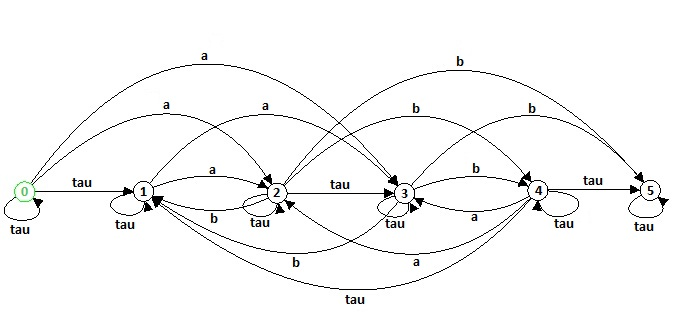
\includegraphics[width=4.5in]{saturation2}
\caption{Example saturated LTS}
\label{fig:saturation2}
\end{figure}